\documentclass[11pt]{article}

% ---------- Page geometry ----------
\usepackage[a4paper,margin=2.6cm,headheight=14pt]{geometry}

% ---------- Fonts (engine-agnostic: works with pdfLaTeX, XeLaTeX, or LuaLaTeX) ----------
\usepackage{iftex}
\ifPDFTeX
  \usepackage[T1]{fontenc}
  \usepackage[utf8]{inputenc}
  \usepackage{textcomp}
  \usepackage{mathptmx}                 % Times-like serif body font
  \usepackage[scaled=0.92]{helvet}      % Helvetica-like sans, used for headings
  \usepackage{courier}                  % monospace fallback for \texttt
\else
  \usepackage{fontspec}
  \setmainfont{TeX Gyre Termes}
  \setsansfont{TeX Gyre Heros}
  \setmonofont{Latin Modern Mono}[Scale=0.92]
\fi

% ---------- Typography ----------
\usepackage{microtype}
\usepackage[english]{babel}
\usepackage{csquotes}
\linespread{1.045}
\frenchspacing

% ---------- Layout helpers ----------
\usepackage{graphicx}
\usepackage{float}          % [H]: place floats exactly where they are defined
\usepackage{booktabs}
\usepackage{array}
\usepackage{tabularx}
\usepackage{longtable}
\usepackage{caption}
\usepackage{subcaption}
\usepackage{xcolor}
\usepackage{enumitem}
\usepackage{titlesec}
\usepackage{fancyhdr}
\usepackage{abstract}
\usepackage[hidelinks,colorlinks=true,linkcolor=black,citecolor=black,urlcolor=teal]{hyperref}
\usepackage[capitalise,nameinlink]{cleveref}
\crefname{figure}{Figure}{Figures}
\Crefname{figure}{Figure}{Figures}
\crefname{table}{Table}{Tables}
\Crefname{table}{Table}{Tables}
\crefname{section}{Section}{Sections}
\Crefname{section}{Section}{Sections}

% ---------- Colours ----------
\definecolor{accent}{HTML}{1f4e5f}
\definecolor{rulegray}{HTML}{8c8c8c}
\definecolor{pidblue}{HTML}{2f6fb0}
\definecolor{losorange}{HTML}{d9702e}
\definecolor{mpcgreen}{HTML}{1f9c76}

% ---------- Section styling ----------
\titleformat{\section}
  {\normalfont\sffamily\Large\bfseries\color{accent}}
  {\thesection}{0.6em}{}
\titleformat{\subsection}
  {\normalfont\sffamily\large\bfseries\color{accent}}
  {\thesubsection}{0.6em}{}
\titlespacing*{\section}{0pt}{1.6em}{0.8em}
\titlespacing*{\subsection}{0pt}{1.2em}{0.5em}

% ---------- Header / footer ----------
\pagestyle{fancy}
\fancyhf{}
\renewcommand{\headrulewidth}{0.4pt}
\renewcommand{\footrulewidth}{0pt}
\fancyhead[L]{\small\sffamily\textcolor{rulegray}{Controller comparison, field trial}}
\fancyhead[R]{\small\sffamily\textcolor{rulegray}{PID / line-of-sight / model-predictive}}
\fancyfoot[C]{\small\sffamily\thepage}

\fancypagestyle{firststyle}{
  \fancyhf{}
  \renewcommand{\headrulewidth}{0pt}
  \fancyfoot[C]{\small\sffamily\thepage}
}

% ---------- Captions ----------
\captionsetup{
  font={small},
  labelfont={bf,sf,color=accent},
  labelsep=colon,
  skip=6pt
}

% ---------- Table column helpers ----------
\newcolumntype{L}[1]{>{\raggedright\arraybackslash}p{#1}}
\newcolumntype{C}[1]{>{\centering\arraybackslash}p{#1}}
\newcolumntype{Y}{>{\raggedright\arraybackslash}X}

% ---------- Small helpers ----------
\newcommand{\ctrl}[1]{\textbf{#1}}
\newcommand{\best}[1]{\textbf{#1}}
\newcommand{\opquote}[1]{%
  \begin{quote}\itshape\small #1\end{quote}%
}

\raggedbottom

\setlength{\parindent}{0pt}
\setlength{\parskip}{0.55em}

\title{\sffamily\bfseries\color{accent}%
  Which controller should steer a survey boat?\\[2pt]
  \Large PID, line-of-sight and model-predictive control compared on the water}

\hypersetup{pdftitle={Which controller should steer a survey boat?}}

\begin{document}

\begin{center}
{\sffamily\bfseries\color{accent}\LARGE
Which controller should steer a survey boat?}\\[6pt]
{\sffamily\bfseries\color{accent}\Large
PID, line-of-sight and model-predictive control compared on the water}
\end{center}
\thispagestyle{firststyle}

\vspace{0.9em}
\begin{center}
\small\sffamily\textcolor{rulegray}{%
36 runs: 4 routes $\times$ 3 controllers, flown in real water and repeated twice in simulation.}
\end{center}

\vspace{0.6em}
\renewcommand{\abstractnamefont}{\normalfont\sffamily\bfseries\color{accent}}
\renewcommand{\abstracttextfont}{\normalfont\small}
\begin{abstract}
\noindent
Three ways of making a BlueBoat follow a planned line were flown back to back over four
routes, then repeated in a simulator with and without a current. Model-predictive control
stayed on average \textbf{0.29\,m} from the planned line against 0.43\,m for PID and 0.40\,m
for line-of-sight; more tellingly, its worst deviation anywhere was \textbf{1.20\,m} against
\textbf{4.79\,m} for PID. It alone finished at the speed the route was planned for, and paid
for that with half as much thrust again per metre. Every number is recomputed from the logs
by \texttt{analyze.py}, re-checked by \texttt{verify.py}, and listed per run in
\texttt{metrics\_all.csv}.
\end{abstract}

% =====================================================================
\section{How the three controllers work}
% =====================================================================

The boat has one thruster on each side: pushing both equally drives it forward, pushing one
harder than the other turns it. Whatever the method, a controller only ever decides two
numbers --- the force asked of each thruster --- twenty times a second, and those forces are
limited to $\pm20$ newtons. If a controller asks for more, \textbf{both} are scaled down by
the same factor rather than cut individually, so the boat still turns the way it intended,
just less forcefully.

None of the three follows a stopwatch. The route is a line drawn on the water with a speed
written along it, and a \textbf{target point slides forward along that line}. It only
advances while the boat is keeping up: more than 3\,m behind and the point stops and waits;
between 0.5\,m and 3\,m behind it moves at a reduced speed; within 0.5\,m it moves at the full
planned speed. This rule is the \textbf{governor}, and it is shared by all three controllers.
A boat can therefore never be abandoned by its own reference --- but one that habitually
trails is handed a permanently slower reference, and the whole survey takes longer. That
turns out to be the largest practical difference between the three.

\begin{table}[H]
\centering
\caption{The three controllers under comparison: what each one looks at on the route, its
governing idea, and the gains actually flown on the physical boat. Gains are the defaults in
\texttt{master\_control.py} for \texttt{isSimulation == False}.}
\label{tab:controllers}
\small
\setlength{\tabcolsep}{4pt}
\begin{tabularx}{\linewidth}{@{} L{1.7cm} Y Y L{5.0cm} @{}}
\toprule
& \textbf{What it looks for on the route} & \textbf{Main idea of the method} & \textbf{Tuning used on the boat} \\
\midrule
\ctrl{PID} &
a point 2.5\,m further along the route than the nearest point, and how far ahead or behind
the boat is along the route &
Two nested stages. The outer pair turns position and heading error into a demanded speed and
turn rate; the inner pair drives the boat onto those demands and sets the thruster forces.
Every loop keeps a running total of past error, so a steady push from wind is eventually
cancelled --- but nothing caps that total. &
Aim-ahead $\Delta = 2.5$\,m.\newline
\emph{Outer $x$} --- along-track error $\to$ speed demand: $k_p\,3.0$, $k_i\,0.01$,
$k_d\,0$.\newline
\emph{Outer $\psi$} --- heading error $\to$ turn-rate demand: $k_p\,3.0$, $k_i\,0.01$,
$k_d\,0$.\newline
\emph{Inner $u$} --- speed error $\to$ forward force: $k_p\,1.0$.\newline
\emph{Inner $r$} --- turn-rate error $\to$ turning moment: $k_p\,1.5$. \\
\addlinespace
\ctrl{Line-of-sight} &
the same point 2.5\,m further along the route, and the speed written on the route there &
One stage, no memory of past error. It steers at the aim-ahead point and asks for the
route's own speed, never for a speed that would close a gap --- so once behind the target
point it matches that point's speed instead of catching up, and settles into a fixed
trailing distance. &
Aim-ahead $\Delta = 2.5$\,m --- the further off the line, the harder it aims
back.\newline
$k_u = 20$ --- forward force per unit of speed error (N per m/s).\newline
$k_\psi = 10$ --- turning moment per unit of heading error.\newline
$k_d = 1.0$ --- turning moment opposing the present turn rate, i.e.\ damping.\newline
Speed scale $= 1.0$ --- the route's own speed is passed through unchanged. \\
\addlinespace
\ctrl{Model-predictive} &
the whole next 2.5\,s of route, in fifteen steps &
It carries a model of how this hull responds to thrust. Every 50\,ms it searches for the
force sequence that keeps the boat closest to that stretch of route for the least thrust,
applies only the first step, then solves again. The force limit sits inside the search, and
planning ahead lets it turn \emph{before} a corner. &
Horizon 15 steps over 2.5\,s, one step every 0.167\,s.\newline
State weights $Q = \mathrm{diag}(50,50,30,1,1,1)$ on $(x, y, \psi, u, v, r)$ --- position and
heading count far above the velocities.\newline
Effort weights $R = \mathrm{diag}(0.015, 0.015)$ on the two thruster forces, as an absolute
penalty with no rate term.\newline
Hard input bounds $\pm20$\,N inside the solver.\newline
Working-set budget 120 iterations, $\max(50,\,4 n_u N)$: the active-set solver needs at least
as many iterations as the condensed problem has variables, or a saturating solve fails
outright.\newline
Plant model 16.01\,kg, 5.64\,kg\,m$^2$ in yaw, with added-mass and damping coefficients
fitted to the hull. \\
\bottomrule
\end{tabularx}
\end{table}

The simulator was run with different tuning for all three controllers. Those values are not
listed here, because \cref{sec:sim} uses simulation only to confirm the ordering of the
methods, not their exact numbers.

% =====================================================================
\section{The four routes}
% =====================================================================

\begin{table}[H]
\centering
\caption{The four planned routes flown by every controller, and the failure mode each one is
designed to expose.}
\label{tab:routes}
\small
\begin{tabularx}{\linewidth}{@{} L{2.6cm} Y L{2.6cm} Y @{}}
\toprule
\textbf{Route} & \textbf{What it looks like} & \textbf{Planned} & \textbf{What it is meant to expose} \\
\midrule
Sine weave & S-shaped weave, 9\,m across, three cycles & 132.2\,m at 0.5\,m/s &
continuously reversing curvature: are the bends cut? \\
Expanding square & square spiral, first side 4\,m, +7\,m each side & 174.5\,m at 0.5\,m/s &
repeated sharp 90\textdegree{} corners: are they overshot? \\
Tough angles & straight leg, 150\textdegree{} arc, long curved sweep & 155.6\,m at
\textbf{0.7\,m/s} & abrupt \emph{changes} of curvature, at the fastest speed \\
Lawnmower & 20 $\times$ 40\,m box, six passes 7\,m apart & 228.1\,m at 0.5\,m/s &
the realistic survey: straights, 180\textdegree{} turns, endurance \\
\bottomrule
\end{tabularx}
\end{table}

% =====================================================================
\section{Where and when the runs were made}
% =====================================================================

\begin{figure}[H]
\centering
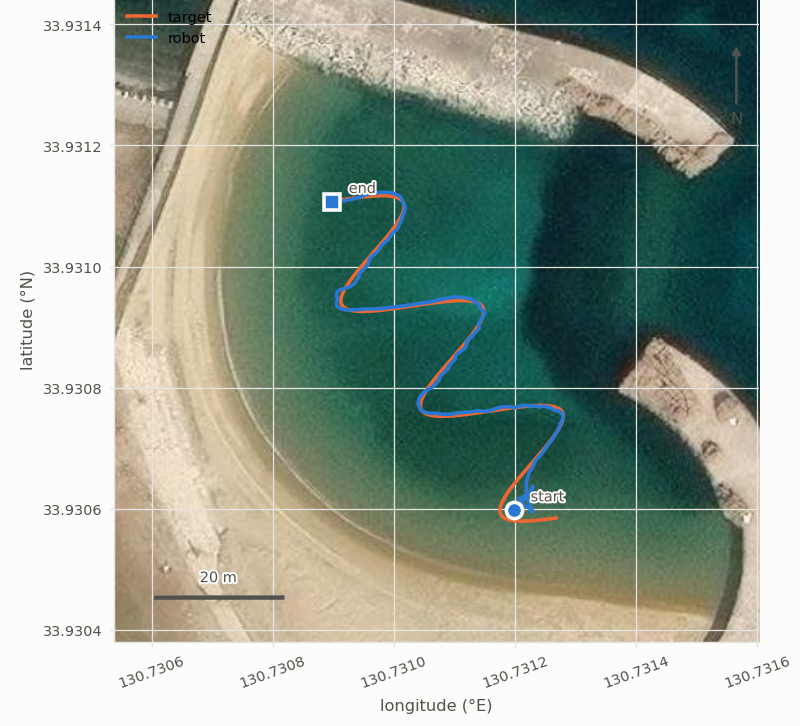
\includegraphics[width=0.62\linewidth]{figures/fig0_site_gps.png}
\caption{\textbf{The field site.} The PID run of the sine weave over satellite imagery. The
basin opens at its \textbf{north-east corner}; wind and flow pushed the boat westward all
day.}
\label{fig:site}
\end{figure}

The twelve field runs were flown back to back between \textbf{10:39 and 12:26}, route by
route (sine weave, expanding square, tough angles, lawnmower) and within each route PID,
then line-of-sight, then model-predictive. The wind blew from the north / north-east all
morning: the Kitakyushu shore record gives a mean of 21\,km/h at 09h, 14\,km/h at 12h and
27\,km/h at 15h, gusting to 35, 22 and 33\,km/h. The basin is semi-enclosed, so waves were
smaller than open sea, but they visibly moved the boat.

\textbf{This is the main weakness of the comparison.} The flow inside the basin cannot be
recovered from a shore wind reading, and the wind roughly halved and then doubled again
across the two hours the runs took, so no two runs met the same conditions. Differences
smaller than the scatter between runs cannot be resolved by this data.

Two things about the boat, in the operator's own words:

\opquote{``In our boat, the right thruster appeared weaker than the left one, but no
compensation gain was used during the field experiments nor simulation, as nothing showed a
need for it. Also, before sending commands to the robot, in case of saturation of the input
(exceeding the $\pm20$\,N limits), a proportional scaling was applied to preserve
direction.''}

Both are confirmed in the flown code: the correction factor is written, then immediately
overwritten with 1.0.

The recordings show that imbalance plainly. The sine weave and the lawnmower turn left as
often as right, so on those two a balanced boat should ask both thrusters for the same
average force. The real boat asked the \textbf{right} thruster for \textbf{2.3 to 3.3
newtons more} than the left; the same two routes in the simulator, where the thrusters are
identical, come out between $-0.4$ and $+0.3$ newtons. The asymmetry is in the boat, and all
three controllers were absorbing it.

% =====================================================================
\section{What happened in real water}
\label{sec:realwater}
% =====================================================================

Two distances appear below and they do \textbf{not} mean the same thing.
\textbf{Distance from the route} --- also called the tracking error --- is measured
sideways, at right angles to the planned line: it says whether the boat actually passed over
the ground the route was drawn across. \textbf{Trailing distance} is how far behind its
moving target point the boat sits; a boat can be exactly on the line and still 1.5\,m from
the target point simply because it is behind it. Trailing costs time, not coverage.

\textbf{Control effort} is the total commanded thruster force, added up over the run and
divided by the metres of route covered, so a slow run is not rewarded for being slow.
\textbf{Accuracy bought with effort} is not a single number: it is those two quantities read
as a pair, as in \cref{fig:tradeoff}(c) --- average distance from the route on the vertical
axis, control effort on the horizontal. Low on the vertical axis means the boat held the
line; far to the right means it burned force to do so. A controller that sits down
\emph{and} to the left is better outright; one that gets down only by moving right is asking
the operator to pay for its accuracy in battery and thruster wear.

\begin{figure}[H]
\centering
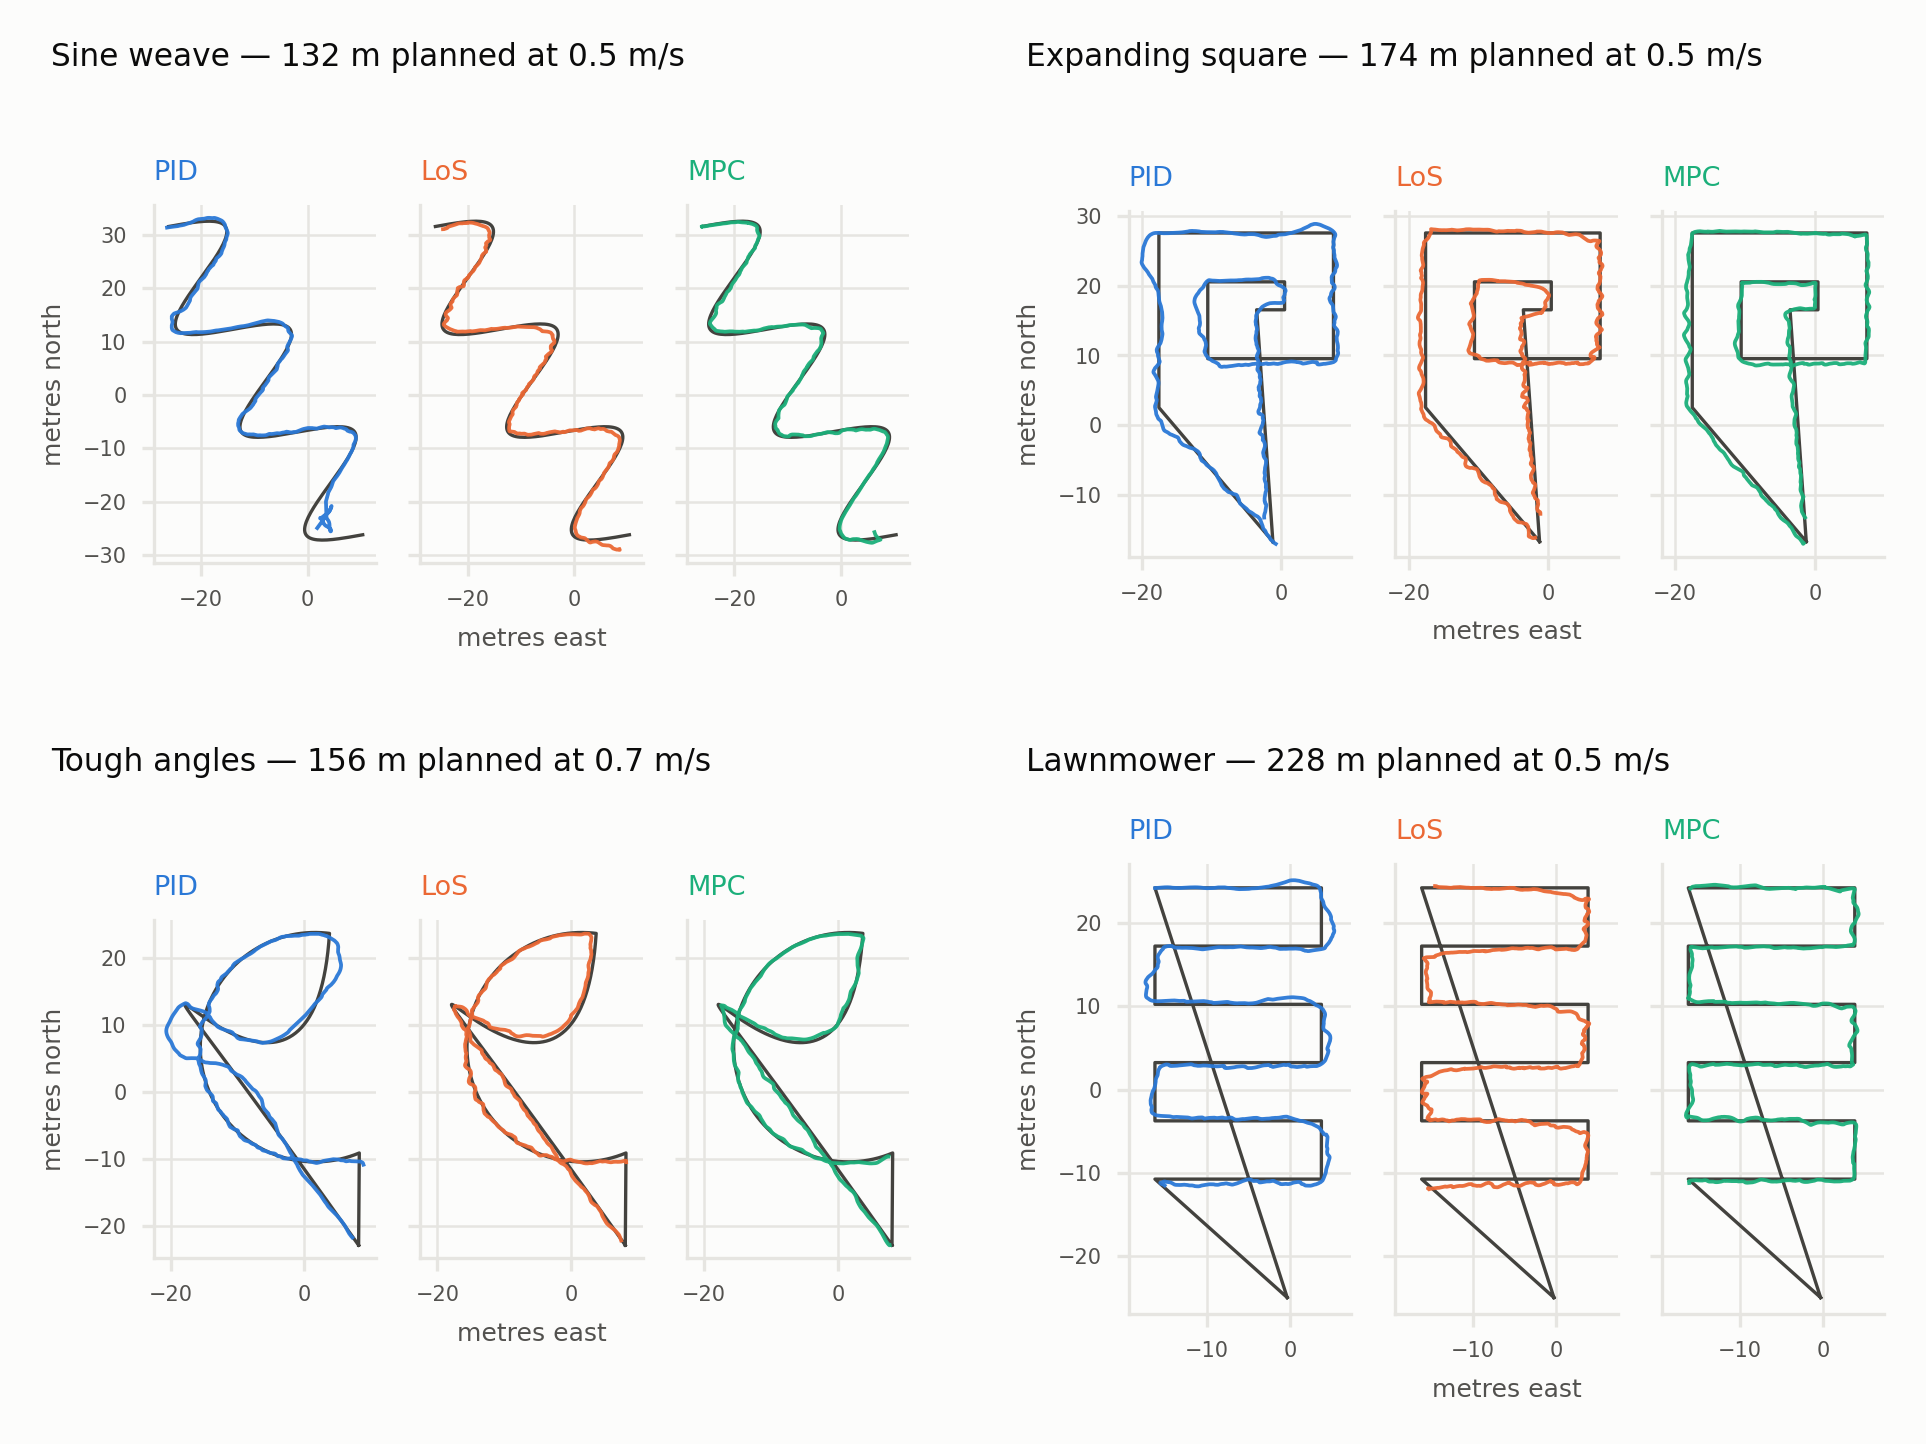
\includegraphics[width=0.98\linewidth]{figures/fig1_trajectories.png}
\caption{\textbf{Planned route against measured track.} All twelve field runs, at true 1:1
scale: four routes, and within each, one small panel per controller. The thin dark line is
the planned route; the coloured line is where the boat actually went. PID's loop at the
start of the sine weave, its overshoot at the corners of the expanding square and its wide
bulge on the 150\textdegree{} arc of the tough-angles route can be read directly.}
\label{fig:traj}
\end{figure}

Tracking figures start from the moment the boat first came within 1\,m of the route, so the
time spent getting onto the line does not contaminate them; how long that took is reported
in \cref{sec:conclusion}.

\begin{table}[H]
\centering
\caption{The twelve field runs. \emph{Average} and \emph{worst} are the sideways distance
from the planned line, in metres. \emph{Over 1\,m} is the share of the run spent further
than a metre from it. \emph{Speed against plan} is progress along the route divided by the
speed it was drawn at, so 100\% means the survey ran to schedule. \emph{Thrust per metre} is
newton-seconds of commanded thrust per metre covered. Best of the three on each route in
bold.}
\label{tab:runs}
\small
\setlength{\tabcolsep}{4.2pt}
\begin{tabular}{@{} L{2.55cm} C{1.15cm} C{1.05cm} C{1.05cm} C{1.75cm} C{1.75cm} C{1.15cm} C{1.0cm} @{}}
\toprule
\textbf{Controller} & \textbf{Average (m)} & \textbf{Worst (m)} & \textbf{Over 1\,m} &
\textbf{Speed against plan} & \textbf{Thrust per metre} & \textbf{Covered} & \textbf{Time} \\
\midrule
\multicolumn{8}{@{}l}{\textit{Sine weave}}\\
PID              & 0.33          & 0.98          & \best{0.0\%} & 79\%          & \best{15.2} & 98\%          & 332\,s \\
Line-of-sight    & 0.34          & 1.37          & 2.9\%        & 66\%          & 16.5        & 99\%          & 393\,s \\
Model-predictive & \best{0.25}   & \best{0.77}   & \best{0.0\%} & \best{99\%}   & 22.0        & \best{99\%}   & \best{265\,s} \\
\addlinespace
\multicolumn{8}{@{}l}{\textit{Expanding square}}\\
PID              & 0.49        & 2.49          & 11.4\%       & 88\%          & \best{15.5} & 98\%          & 389\,s \\
Line-of-sight    & 0.47        & 1.30          & 4.1\%        & 65\%          & 17.6        & 97\%          & 523\,s \\
Model-predictive & \best{0.41} & \best{1.20}   & \best{1.3\%} & \best{99\%}   & 25.5        & \best{98\%}   & \best{346\,s} \\
\addlinespace
\multicolumn{8}{@{}l}{\textit{Tough angles}}\\
PID              & 0.46        & 4.79          & 9.7\%        & 74\%          & 14.8        & 90\%          & 272\,s \\
Line-of-sight    & 0.32        & 1.03          & 0.4\%        & 65\%          & \best{13.1} & 91\%          & 312\,s \\
Model-predictive & \best{0.27} & \best{0.80}   & \best{0.0\%} & \best{100\%}  & 19.8        & \best{92\%}   & \best{204\,s} \\
\addlinespace
\multicolumn{8}{@{}l}{\textit{Lawnmower}}\\
PID              & 0.42        & 1.54          & 4.0\%        & 85\%          & \best{16.3} & 68\%          & 365\,s \\
Line-of-sight    & 0.47        & 1.47          & 5.9\%        & 62\%          & 19.6        & 68\%          & 492\,s \\
Model-predictive & \best{0.24} & \best{0.63}   & \best{0.0\%} & \best{99\%}   & 30.2        & 68\%          & \best{313\,s} \\
\bottomrule
\end{tabular}
\end{table}

\begin{figure}[H]
\centering
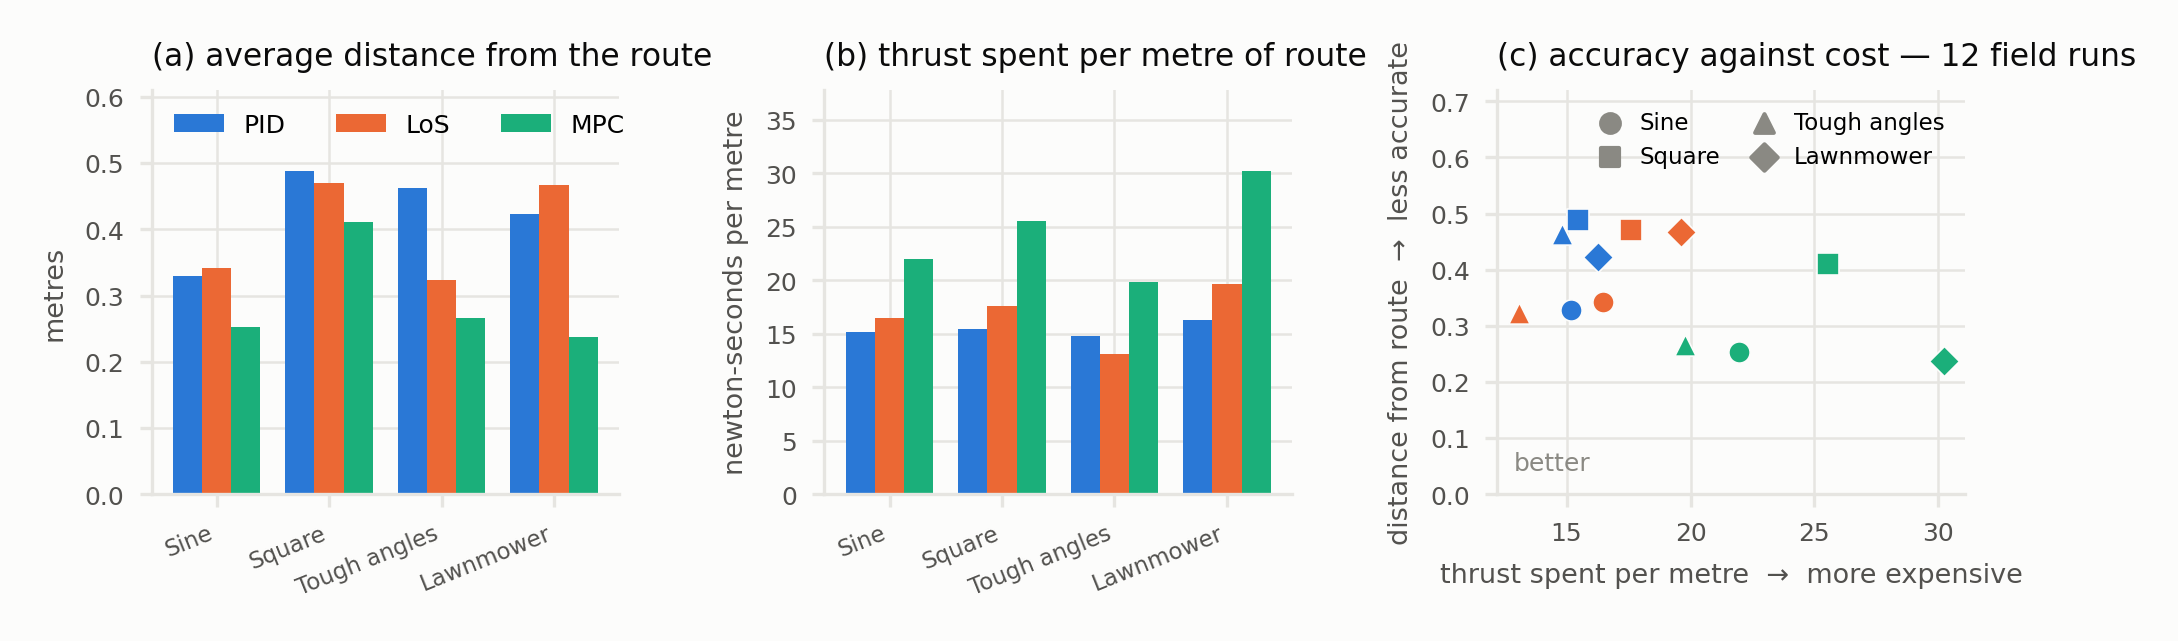
\includegraphics[width=0.98\linewidth]{figures/fig2_tradeoff.png}
\caption{\textbf{Accuracy, cost, and the trade between them.} Field runs only.
\textbf{(a)} average distance from the planned route and \textbf{(b)} thrust spent per
metre, by route and controller. \textbf{(c)} the same twelve runs with the two against each
other: lower is closer to the route, further right is more force spent, so the bottom-left
corner is the best place to be.}
\label{fig:tradeoff}
\end{figure}

\textbf{Why two of the three finish late.} The governor is the reason. A controller that
sits well behind its target point is in effect telling the governor to slow down, and the
governor obliges for the rest of the run. Model-predictive control never falls behind --- it
sits a fraction of a metre \emph{in front} of its target point --- so it is never throttled
and covers the route at the speed the route was drawn for. PID sits 0.7 to 1.2\,m back and
gets 74--88\% of that speed. Line-of-sight sits 1.3 to 1.4\,m back, by design rather than by
accident, and gets 62--66\%. The link is tight enough to check directly: take each run's
measured trailing distance, put it into the governor's rule, and the speed it predicts
matches the speed the run actually achieved to within 5\%, in all twelve field runs. The
cost shows up at the end of the day rather than in the track --- the same four routes took
\textbf{1128\,s with model-predictive control, 1358\,s with PID (20\% longer) and 1721\,s
with line-of-sight (53\% longer)}.

\textbf{The boat was being shaken, and the controllers were not doing it.} In the field the
hull rolled with a standard deviation of 1.6--2.6\textdegree{} and its roll rate averaged
0.15--0.24\,rad/s; in both simulations, which contain no waves, those figures are
0.13--0.28\textdegree{} and 0.003\,rad/s --- sixty times smaller, with a clear field rhythm
near one cycle per second that is short wind chop rather than swell. The boat also reversed
its turning direction 7 to 26 times a minute in the field against 0.2 to 5.4 in simulation,
for all three controllers alike, so those reversals are the sea moving the boat, not a
controller hunting.

\begin{figure}[H]
\centering
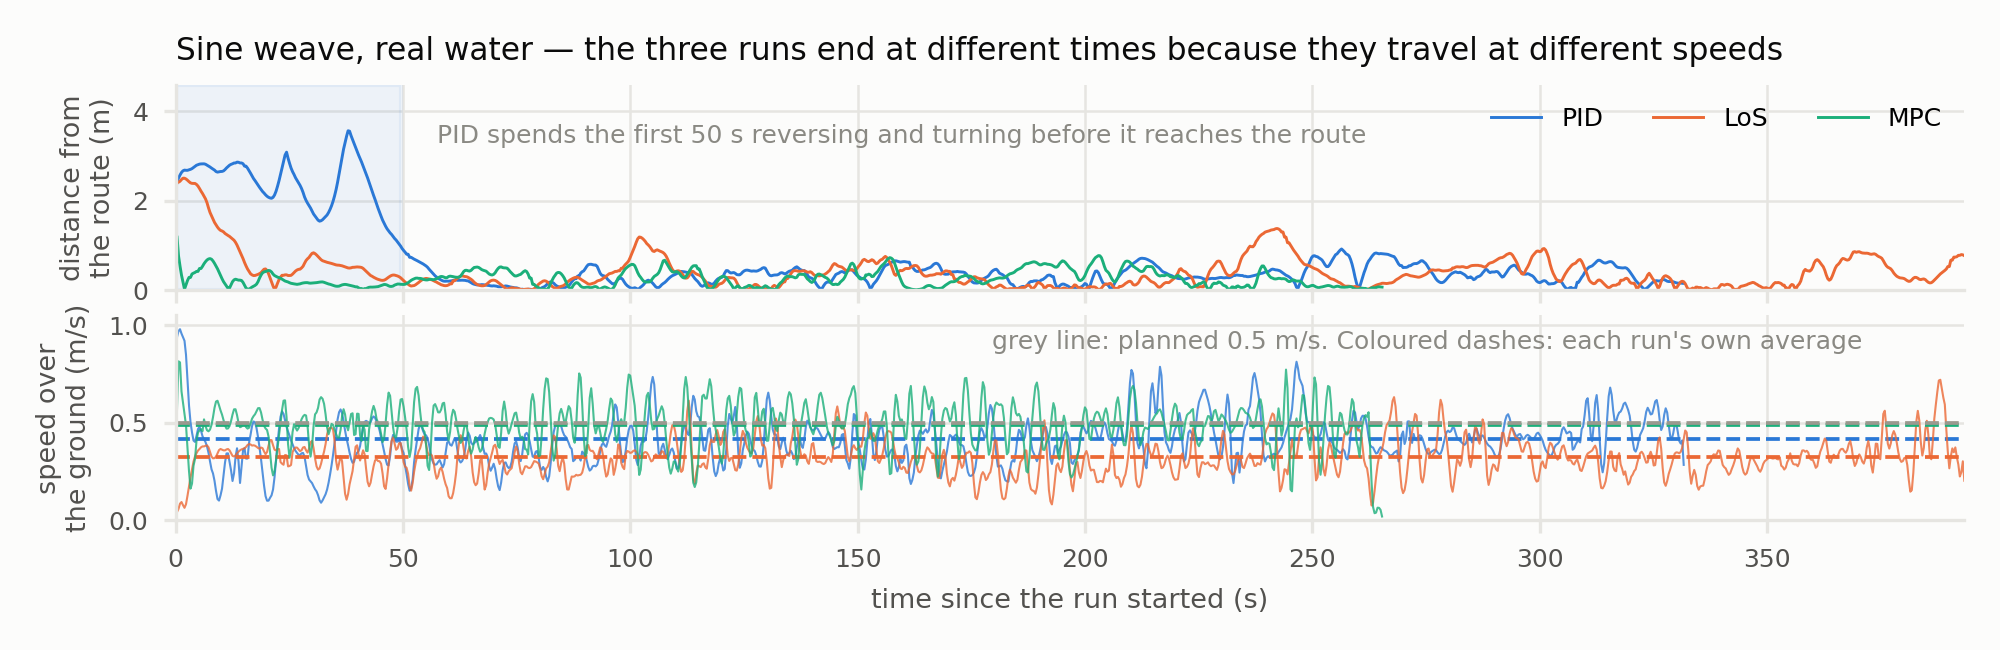
\includegraphics[width=0.98\linewidth]{figures/fig3_timeseries_sin.png}
\caption{\textbf{One route, second by second.} The sine weave in real water. Top: distance
from the planned route. Bottom: speed, each run's average dashed in its own colour, the
planned 0.5\,m/s in grey.}
\label{fig:timeseries}
\end{figure}

% =====================================================================
\section{Does the simulator agree?}
\label{sec:sim}
% =====================================================================

The twelve missions were repeated twice in Gazebo: once in calm water, once with a current
of about 0.1\,m/s running north-north-east to south-south-west, worth roughly 2.5\,N of drag
on a stationary boat.

\begin{table}[H]
\centering
\caption{Field and simulated performance, averaged over the four routes. Best of the three
controllers in each row in bold.}
\label{tab:sim}
\small
\begin{tabular}{@{} L{6.6cm} C{1.7cm} C{1.9cm} C{2.3cm} @{}}
\toprule
\textbf{Averaged over the four routes} & \textbf{PID} & \textbf{Line-of-sight} & \textbf{Model-predictive} \\
\midrule
Average distance from the route, real water (m) & 0.43 & 0.40 & \best{0.29} \\
\quad\ldots{} in calm simulation & 0.18 & \best{0.07} & \best{0.07} \\
\quad\ldots{} in simulation with a current & 0.39 & 0.42 & \best{0.18} \\
\addlinespace
Thrust per metre, real water & \best{15.4} & 16.7 & 24.4 \\
\quad\ldots{} in calm simulation & 41.1 & \best{38.4} & 43.6 \\
\quad\ldots{} in simulation with a current & 44.0 & \best{41.8} & 46.6 \\
\addlinespace
Speed against plan, real water & 81\% & 64\% & \best{99\%} \\
\quad\ldots{} in calm simulation & 78\% & 70\% & \best{99\%} \\
\quad\ldots{} in simulation with a current & 75\% & 67\% & \best{94\%} \\
\bottomrule
\end{tabular}
\end{table}

Four things carry across. The \textbf{ordering holds} in all three conditions:
model-predictive control the most accurate and most expensive, line-of-sight the cheapest.
The \textbf{speed penalty transfers exactly} --- each controller's share of the planned
speed moves by at most 0.07 between real water and either simulation, confirming it comes
from the governor, not from the weather. \textbf{Calm simulation is far too optimistic}, by
two to six times; adding the current brings the errors back into the measured range, hurting
line-of-sight most (0.07 $\rightarrow$ 0.42\,m) and model-predictive control least
(0.07 $\rightarrow$ 0.18\,m). And \textbf{PID's weakness is the controller, not the
weather}: in calm simulation, with no wind and no waves at all, it still goes
\textbf{4.76\,m} off the tough-angles route --- within three centimetres of the 4.79\,m it
managed in the field --- and it is the only one of the three that ever exceeds a metre in
calm water.

One caveat in PID's favour: its simulated gains were never re-tuned for the simulated hull,
so part of its poor showing in simulation is tuning rather than method, and a proper re-tune
there would likely close some of that gap. It would not close the part that also appears in
the field, where the gains \emph{were} tuned for the real boat.

% =====================================================================
\section{What to choose}
% =====================================================================

\begin{table}[H]
\centering
\caption{Recommended controller by route, with a fallback where the force budget is tight.}
\label{tab:choice}
\small
\begin{tabularx}{\linewidth}{@{} L{2.6cm} L{2.6cm} Y L{1.5cm} @{}}
\toprule
\textbf{Route} & \textbf{Recommended} & \textbf{Fallback if the force budget is tight} & \textbf{Avoid} \\
\midrule
Sine weave & model-predictive & PID: as accurate as line-of-sight here, and 15\% faster & --- \\
Expanding square & model-predictive & line-of-sight: PID overshoots the corners & PID \\
Tough angles & model-predictive & line-of-sight: cheapest of all twelve runs, within
0.05\,m of the best & PID \\
Lawnmower & model-predictive & PID: cheaper and more accurate here than line-of-sight & --- \\
\bottomrule
\end{tabularx}
\end{table}

\emph{What this comparison cannot tell you.} One site, one day, one run per combination,
with the wind changing by a factor of two across the two hours --- so any difference smaller
than the scatter between runs is not resolvable here. The simulator used different gains and
hull model, so it supports the ordering of the methods and nothing finer. Positions were
logged three times a second, making the command-activity figures a lower bound. The three
lawnmower runs were all stopped at the same 68\% of the route: comparable with one another,
but none is a completed survey.

% =====================================================================
\section{Detailed conclusion}
\label{sec:conclusion}
% =====================================================================

\textbf{Choose model-predictive control wherever the boat's power and thruster budget allow
it.} The case is not marginal. It was the most accurate on every route (0.24--0.41\,m
average, against 0.33--0.49\,m for PID and 0.32--0.47\,m for line-of-sight); its worst
moment anywhere was 1.20\,m against PID's 4.79\,m; it reached the line within 0.7\,s of every
start; and it is the only controller that never spent a measurable part of a run more than a
metre off the line. How much that matters depends on what the boat is carrying, and coverage
is the clearest example: the lawnmower's passes were set 7\,m apart so that the swaths of the
\textbf{side-scan sonar mounted on the USV} overlap from one pass to the next. A controller
whose bad moments stay near 0.5\,m keeps that overlap intact, whereas PID's single 4.79\,m
excursion is more than half a line spacing --- a strip of ground left unimaged rather than a
cosmetic blemish. And because it alone holds the planned speed, the same four routes finished
\textbf{20\% sooner than with PID and 53\% sooner than with line-of-sight}, which on a
weather-limited field day converts directly into more lines covered.

\textbf{What it costs is wear and power, not accuracy.} Model-predictive control spends
24.4\,newton-seconds of thrust per metre against 15.4 for PID and 16.7 for line-of-sight,
commands roughly twice the total thrust, changes its command about thirteen times more often
than PID, and sits at the $\pm20$\,N limit for 7.8\% of an average run and 13.9\% of the
lawnmower. It is the only one working near the limits of the thrusters, and the only one
whose cost climbs steeply with how much turning a route demands --- 19.8\,newton-seconds per
metre on the tough-angles route against 30.2 on the lawnmower. It also needs an optimisation
solved every 50\,ms where the other two need a few lines of arithmetic, which is a real
constraint if the controller must ever move to a smaller on-board computer.

\textbf{Where endurance, thruster wear or a tight force budget dominates, use
line-of-sight.} It is the cheapest and the most even-tempered of the three: it produced no
large excursion on any route, and on the tough-angles route it was at once the cheapest run
of the campaign and within 0.05\,m of the best accuracy measured. Its price is explicit and
permanent, and it is a property of the method rather than of its tuning --- with no memory of
past error and a forward speed copied from the route instead of computed to close a gap, it
settles 1.3--1.4\,m behind its target point, and the governor turns that into a mission
roughly a third longer. If the survey is limited by daylight or weather rather than by
battery, that is the wrong trade.

\textbf{Use PID only on gentle routes.} It is the cheapest on three routes out of four and
the better classical method on the sine weave, where it is as accurate as line-of-sight and
15\% faster. But it is the only controller that produced deviations beyond 2\,m, and it did
so on two different routes; on the expanding square it spent 11.4\% of the run more than a
metre off the line, overshooting the corners. It is also the least dependable at the start:
the operator's note on the sine weave describes exactly what the top panel of
\cref{fig:timeseries} shows ---

\opquote{``Notice that PID struggled at the beginning: it made the robot going backward +
rotating before finally reaching the path''}

--- and it took 50\,s to get onto the line, against 0.7\,s for model-predictive control. This
happens intermittently with this controller and is consistent with its running totals of
past error, which have no ceiling and can build up while the boat is still far away. Calm
simulation reproduces its worst field excursion to within three centimetres, so better
weather will not fix it.

\end{document}